\chapter{Details on the smooth transition function} \label{sec:smooth-transition}    
    To mathematically define an expression for $\Psi(\vec{x})$ in \S\ref{sec:modelling:blood-flow}, we first introduce some auxiliary variables. The simple idea here is that we assign $\Psi = 1$ in areas of villous tree and $\Psi = 0$ in areas of no villous tree.    
    
    The central cavity is defined by half an ellipse (a semi-ellipse) with a semi-minor axis of $a_1$ and a semi-major axis of $b_1$, where $2a_1 = b_1$ with $a_1$ denoting the semi-axis that is tangential to the basal plate. We then add two more ellipses at equal distances inside and outside the first ellipse, which acts as a transition region. We introduce a smooth transition function defined as
    \begin{equation}
        \beta_{s_0,s_1,s_2}(s) := 
        \begin{cases}
            0 & \text{if } 0 \leq s < s_0, \\
            \frac{1}{2}\left[ \frac{\tanh(\gamma\left\{ \frac{s-s_1}{s_2-s_1} \right\})}{\tanh(\gamma)} + 1 \right], & \text{if } s_0 \leq s \leq s_2, \\
            1 & \text{if } s_2 < s, \\
        \end{cases}
    \end{equation}
    where $s_2 - s_0$ gives the transition width, and we assume the relation $s_1 \equiv \frac{s_0 + s_2}{2}$. We note that $\beta$ differs from $\tanh$, as $\tanh$ has asymptotes at $\pm 1$, whereas $\beta$ has no such asymptotes; $\beta$ instead attains maximum and minimum values by taking a `cut-off' value, parameterised by $\gamma$, outside which $\beta$ attains its extrema. We note that the scaling $\gamma$ is included so that $\beta$ is continuous everywhere, and is fixed $\gamma = 0.999$. These differences are illustrated in Figure \ref{fig:transition:beta}.

    \begin{figure}
        \begin{subfigure}[b]{0.45\textwidth}
            \centering
            

\tikzset{every picture/.style={line width=0.75pt}} %set default line width to 0.75pt        

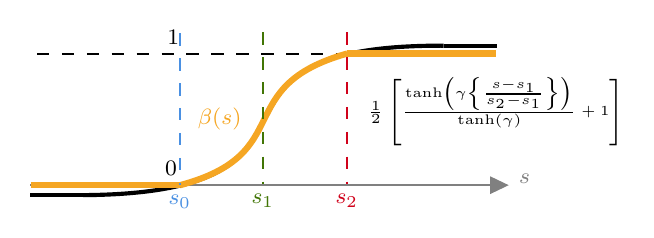
\begin{tikzpicture}[x=0.75pt,y=0.75pt,yscale=-1,xscale=1]
%uncomment if require: \path (0,215); %set diagram left start at 0, and has height of 215

%Straight Lines [id:da46631770507939163] 
\draw [color={rgb, 255:red, 128; green, 128; blue, 128 }  ,draw opacity=1 ]   (23,143.86) -- (250.5,143.86) ;
\draw [shift={(253.5,143.86)}, rotate = 180] [fill={rgb, 255:red, 128; green, 128; blue, 128 }  ,fill opacity=1 ][line width=0.08]  [draw opacity=0] (8.93,-4.29) -- (0,0) -- (8.93,4.29) -- cycle    ;
%Curve Lines [id:da39491275569940676] 
\draw [color={rgb, 255:red, 0; green, 0; blue, 0 }  ,draw opacity=1 ][line width=1.5]    (222.18,76.65) .. controls (87,76.16) and (185,147.66) .. (48.5,148.66) ;
%Straight Lines [id:da15611460318667292] 
\draw [color={rgb, 255:red, 0; green, 0; blue, 0 }  ,draw opacity=1 ][line width=1.5]    (23,148.66) -- (48.5,148.66) ;
%Straight Lines [id:da034171139038229326] 
\draw [color={rgb, 255:red, 0; green, 0; blue, 0 }  ,draw opacity=1 ][line width=1.5]    (222.18,76.65) -- (247.68,76.65) ;
%Straight Lines [id:da7075728897093001] 
\draw  [dash pattern={on 4.5pt off 4.5pt}]  (26.25,80.5) -- (247.25,80.5) ;
%Straight Lines [id:da5994500046428453] 
\draw [color={rgb, 255:red, 208; green, 2; blue, 27 }  ,draw opacity=1 ] [dash pattern={on 4.5pt off 4.5pt}]  (175.5,70.16) -- (175.5,143.41) ;
%Curve Lines [id:da28483688604328905] 
\draw [color={rgb, 255:red, 245; green, 166; blue, 35 }  ,draw opacity=1 ][line width=2.25]    (175.75,80.41) .. controls (119,96.41) and (152.25,128.66) .. (95,143.91) ;
%Straight Lines [id:da5305187515219363] 
\draw [color={rgb, 255:red, 245; green, 166; blue, 35 }  ,draw opacity=1 ][line width=2.25]    (175.75,80.41) -- (247.5,80.41) ;
%Straight Lines [id:da005336188299916778] 
\draw [color={rgb, 255:red, 245; green, 166; blue, 35 }  ,draw opacity=1 ][line width=2.25]    (23.25,143.91) -- (95,143.91) ;
%Straight Lines [id:da5146644196761871] 
\draw [color={rgb, 255:red, 65; green, 117; blue, 5 }  ,draw opacity=1 ] [dash pattern={on 4.5pt off 4.5pt}]  (135,70.16) -- (135,143.41) ;
%Straight Lines [id:da581762102800299] 
\draw [color={rgb, 255:red, 74; green, 144; blue, 226 }  ,draw opacity=1 ] [dash pattern={on 4.5pt off 4.5pt}]  (95,70.66) -- (95,143.91) ;

% Text Node
\draw (256.99,136.89) node [anchor=north west][inner sep=0.75pt]  [font=\footnotesize,color={rgb, 255:red, 128; green, 128; blue, 128 }  ,opacity=1 ]  {$s$};
% Text Node
\draw (114.25,118.76) node [anchor=south] [inner sep=0.75pt]  [font=\footnotesize,color={rgb, 255:red, 245; green, 166; blue, 35 }  ,opacity=1 ]  {$\beta ( s)$};
% Text Node
\draw (96.25,77.35) node [anchor=south east] [inner sep=0.75pt]  [font=\footnotesize]  {$1$};
% Text Node
\draw (95.19,140.6) node [anchor=south east] [inner sep=0.75pt]  [font=\footnotesize]  {$0$};
% Text Node
\draw (175.5,146.81) node [anchor=north] [inner sep=0.75pt]  [font=\footnotesize,color={rgb, 255:red, 208; green, 2; blue, 27 }  ,opacity=1 ]  {$s_{2}$};
% Text Node
\draw (184.07,108.31) node [anchor=west] [inner sep=0.75pt]  [font=\tiny,color={rgb, 255:red, 0; green, 0; blue, 0 }  ,opacity=1 ]  {$\frac{1}{2}\left[\frac{\tanh\left( \gamma \left\{\frac{s-s_{1}}{s_{2} -s_{1}}\right\}\right)}{\tanh( \gamma )} +1\right]$};
% Text Node
\draw (135,146.81) node [anchor=north] [inner sep=0.75pt]  [font=\footnotesize,color={rgb, 255:red, 65; green, 117; blue, 5 }  ,opacity=1 ]  {$s_{1}$};
% Text Node
\draw (95,147.31) node [anchor=north] [inner sep=0.75pt]  [font=\footnotesize,color={rgb, 255:red, 74; green, 144; blue, 226 }  ,opacity=1 ]  {$s_{0}$};


\end{tikzpicture}

            \caption{}
            \label{fig:transition:beta}
        \end{subfigure}
        \hfill
        \begin{subfigure}[b]{0.45\textwidth}
            \centering
            

\tikzset{every picture/.style={line width=0.75pt}} %set default line width to 0.75pt        

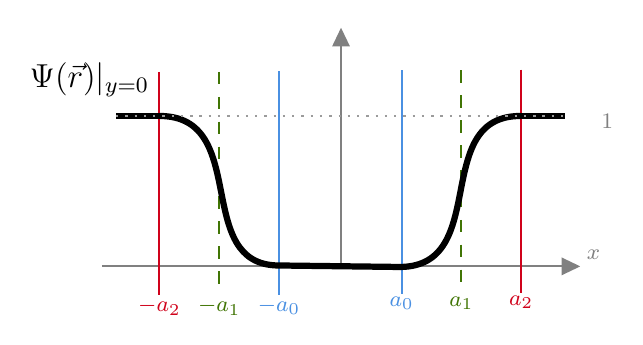
\begin{tikzpicture}[x=0.75pt,y=0.75pt,yscale=-1,xscale=1]
%uncomment if require: \path (0,216); %set diagram left start at 0, and has height of 216

%Straight Lines [id:da6021526004344566] 
\draw [color={rgb, 255:red, 128; green, 128; blue, 128 }  ,draw opacity=1 ]   (191.25,165.61) -- (191.25,53.66) ;
\draw [shift={(191.25,50.66)}, rotate = 90] [fill={rgb, 255:red, 128; green, 128; blue, 128 }  ,fill opacity=1 ][line width=0.08]  [draw opacity=0] (8.93,-4.29) -- (0,0) -- (8.93,4.29) -- cycle    ;
%Straight Lines [id:da09217173902055342] 
\draw [color={rgb, 255:red, 128; green, 128; blue, 128 }  ,draw opacity=1 ]   (76,165.61) -- (303.5,165.61) ;
\draw [shift={(306.5,165.61)}, rotate = 180] [fill={rgb, 255:red, 128; green, 128; blue, 128 }  ,fill opacity=1 ][line width=0.08]  [draw opacity=0] (8.93,-4.29) -- (0,0) -- (8.93,4.29) -- cycle    ;
%Straight Lines [id:da17327433842972684] 
\draw [color={rgb, 255:red, 74; green, 144; blue, 226 }  ,draw opacity=1 ]   (220.42,71.18) -- (220.42,178.87) ;
%Straight Lines [id:da5164207646575634] 
\draw [color={rgb, 255:red, 65; green, 117; blue, 5 }  ,draw opacity=1 ] [dash pattern={on 4.5pt off 4.5pt}]  (249.23,71.18) -- (249.23,178.87) ;
%Straight Lines [id:da9169226167412352] 
\draw [color={rgb, 255:red, 208; green, 2; blue, 27 }  ,draw opacity=1 ]   (278.04,70.82) -- (278.04,178.51) ;
%Straight Lines [id:da08965664307645271] 
\draw [color={rgb, 255:red, 208; green, 2; blue, 27 }  ,draw opacity=1 ]   (103.73,71.91) -- (103.73,179.59) ;
%Straight Lines [id:da855492609907931] 
\draw [color={rgb, 255:red, 65; green, 117; blue, 5 }  ,draw opacity=1 ] [dash pattern={on 4.5pt off 4.5pt}]  (132.54,71.91) -- (132.54,179.59) ;
%Straight Lines [id:da32654209361141806] 
\draw [color={rgb, 255:red, 74; green, 144; blue, 226 }  ,draw opacity=1 ]   (161.36,71.54) -- (161.36,179.23) ;
%Curve Lines [id:da03668323289068964] 
\draw [line width=2.25]    (104.09,93.15) .. controls (148.03,93.51) and (119.22,165.18) .. (161.36,165.18) ;
%Curve Lines [id:da11356455536917842] 
\draw [line width=2.25]    (277.68,93.15) .. controls (234.11,93.15) and (263.64,165.54) .. (219.7,165.9) ;
%Straight Lines [id:da3940509531593688] 
\draw [line width=2.25]    (161.36,165.18) -- (219.7,165.9) ;
%Straight Lines [id:da4374758728023367] 
\draw [line width=2.25]    (277.68,93.15) -- (298.93,93.15) ;
%Straight Lines [id:da7083449686833048] 
\draw [line width=2.25]    (82.84,93.15) -- (104.09,93.15) ;
%Straight Lines [id:da2928034275546325] 
\draw [color={rgb, 255:red, 155; green, 155; blue, 155 }  ,draw opacity=1 ][line width=0.75]  [dash pattern={on 0.84pt off 2.51pt}]  (82.84,93.15) -- (298,93.15) ;

% Text Node
\draw (308.24,156.39) node [anchor=north west][inner sep=0.75pt]  [font=\footnotesize,color={rgb, 255:red, 128; green, 128; blue, 128 }  ,opacity=1 ]  {$x$};
% Text Node
\draw (100.22,85.51) node [anchor=south east] [inner sep=0.75pt]  [font=\large,color={rgb, 255:red, 0; green, 0; blue, 0 }  ,opacity=1 ]  {$\Psi(\vec{r}) |_{y=0}$};
% Text Node
\draw (220.42,178.91) node [anchor=north] [inner sep=0.75pt]  [font=\footnotesize,color={rgb, 255:red, 74; green, 144; blue, 226 }  ,opacity=1 ]  {$a_{0}$};
% Text Node
\draw (249.23,178.91) node [anchor=north] [inner sep=0.75pt]  [font=\footnotesize,color={rgb, 255:red, 65; green, 117; blue, 5 }  ,opacity=1 ]  {$a_{1}$};
% Text Node
\draw (278.04,178.55) node [anchor=north] [inner sep=0.75pt]  [font=\footnotesize,color={rgb, 255:red, 208; green, 2; blue, 27 }  ,opacity=1 ]  {$a_{2}$};
% Text Node
\draw (161.36,179.27) node [anchor=north] [inner sep=0.75pt]  [font=\footnotesize,color={rgb, 255:red, 74; green, 144; blue, 226 }  ,opacity=1 ]  {$-a_{0}$};
% Text Node
\draw (132.54,179.63) node [anchor=north] [inner sep=0.75pt]  [font=\footnotesize,color={rgb, 255:red, 65; green, 117; blue, 5 }  ,opacity=1 ]  {$-a_{1}$};
% Text Node
\draw (103.73,179.63) node [anchor=north] [inner sep=0.75pt]  [font=\footnotesize,color={rgb, 255:red, 208; green, 2; blue, 27 }  ,opacity=1 ]  {$-a_{2}$};
% Text Node
\draw (319.5,100.76) node [anchor=south] [inner sep=0.75pt]  [font=\footnotesize,color={rgb, 255:red, 128; green, 128; blue, 128 }  ,opacity=1 ]  {$1$};


\end{tikzpicture}

            \caption{}
            \label{fig:transition:slice}
        \end{subfigure}
        \caption{(a) Curve of $\beta(s)$ in relation to $s_0$, $s_1$, and $s_2$. (b) Curve showing a slice of $\Psi$ on a placentone along $y = 0$ (i.e. on the basal plate) at the bottom of the cavity region, where $a_0$, $a_1$, and $a_2$ respectively denote the semi-minor axes of the inner, centre, and outer ellipses.}
        \label{fig:transition}
    \end{figure}

    The ellipses which form the geometry of the smooth transition region at the boundary of the central cavity are defined by
    \begin{align}
        \begin{split}
            r_0(\theta) & := \frac{a_0 b_0}{\sqrt{a_0^2 \sin^2(\theta) + b_0^2 \cos^2(\theta)}},
        \end{split}\\
        \begin{split}
            r_1(\theta) & := \frac{a_1 b_1}{\sqrt{a_1^2 \sin^2(\theta) + b_1^2 \cos^2(\theta)}},
        \end{split}\\
        \begin{split}
            r_2(\theta) & := \frac{a_2 b_2}{\sqrt{a_2^2 \sin^2(\theta) + b_2^2 \cos^2(\theta)}},
        \end{split}
    \end{align}
    where $\vec{x} \equiv (x, y)^\intercal$ are 2D Cartesian coordinates, and
    \begin{align}
        \begin{split}
            \theta(\vec{x}) & := \arctan{\left(\frac{y-c_2}{x-c_1}\right)},
        \end{split}\\
        \begin{split}
            r(\vec{x}) & := \sqrt{(\vec{x} - \vec{c}) \cdot (\vec{x} - \vec{c})}
        \end{split}
    \end{align}
    are 2D polar coordinates with $r = 0$ at $\vec{c} \equiv (c_1, c_2)^\intercal$ and $\theta = 0$ is tangential to the interface between $\Omega_\text{CC}$ and $\Omega_\text{a}$ (pointing in the anticlockwise direction). Here, $\vec{c}$ is the point at the centre of where an artery meets the placenta. The transition width, $\tau$, is defined such that $\tau = a_2 - a_0$ and $2\tau = b_2 - b_0$. The transition region in the central cavity is illustrated in Figure \ref{fig:transition-sizes:cavity}.

    \begin{figure}
        \begin{subfigure}[b]{0.45\textwidth}
            \centering
            

\tikzset{every picture/.style={line width=0.75pt}} %set default line width to 0.75pt        

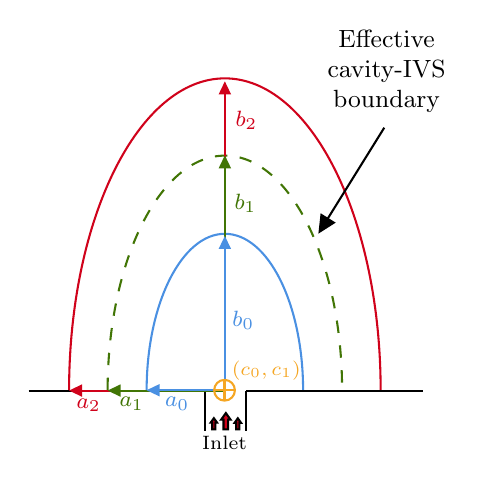
\begin{tikzpicture}[x=0.75pt,y=0.75pt,yscale=-1,xscale=1]
%uncomment if require: \path (0,300); %set diagram left start at 0, and has height of 300

%Shape: Arc [id:dp03766549009182518] 
\draw  [draw opacity=0] (43.89,241.51) .. controls (43.97,158.57) and (77.54,91.4) .. (118.94,91.4) .. controls (160.34,91.4) and (193.92,158.57) .. (194,241.51) -- (118.94,241.82) -- cycle ; \draw  [color={rgb, 255:red, 208; green, 2; blue, 27 }  ,draw opacity=1 ] (43.89,241.51) .. controls (43.97,158.57) and (77.54,91.4) .. (118.94,91.4) .. controls (160.34,91.4) and (193.92,158.57) .. (194,241.51) ;  
%Straight Lines [id:da2354434472901965] 
\draw    (109.5,241.82) -- (109.5,261.48) ;
%Straight Lines [id:da5144009246972279] 
\draw    (24.44,241.82) -- (108.75,241.82) ;
%Shape: Arc [id:dp18686074775091321] 
\draw  [draw opacity=0][dash pattern={on 4.5pt off 4.5pt}] (62.46,241.59) .. controls (62.52,179.17) and (87.79,128.62) .. (118.94,128.62) .. controls (150.1,128.62) and (175.36,179.17) .. (175.43,241.59) -- (118.94,241.82) -- cycle ; \draw  [color={rgb, 255:red, 65; green, 117; blue, 5 }  ,draw opacity=1 ][dash pattern={on 4.5pt off 4.5pt}] (62.46,241.59) .. controls (62.52,179.17) and (87.79,128.62) .. (118.94,128.62) .. controls (150.1,128.62) and (175.36,179.17) .. (175.43,241.59) ;  
%Shape: Arc [id:dp32870840671183665] 
\draw  [draw opacity=0] (81.25,241.66) .. controls (81.29,200.01) and (98.15,166.28) .. (118.94,166.28) .. controls (139.73,166.28) and (156.6,200.01) .. (156.64,241.66) -- (118.94,241.82) -- cycle ; \draw  [color={rgb, 255:red, 74; green, 144; blue, 226 }  ,draw opacity=1 ] (81.25,241.66) .. controls (81.29,200.01) and (98.15,166.28) .. (118.94,166.28) .. controls (139.73,166.28) and (156.6,200.01) .. (156.64,241.66) ;  
%Straight Lines [id:da13365761646036511] 
\draw [color={rgb, 255:red, 208; green, 2; blue, 27 }  ,draw opacity=1 ]   (118.94,241.82) -- (118.94,95.85) ;
\draw [shift={(118.94,92.85)}, rotate = 90] [fill={rgb, 255:red, 208; green, 2; blue, 27 }  ,fill opacity=1 ][line width=0.08]  [draw opacity=0] (6.25,-3) -- (0,0) -- (6.25,3) -- cycle    ;
%Straight Lines [id:da12333016540641895] 
\draw [color={rgb, 255:red, 208; green, 2; blue, 27 }  ,draw opacity=1 ]   (118.94,241.82) -- (46.89,241.82) ;
\draw [shift={(43.89,241.82)}, rotate = 360] [fill={rgb, 255:red, 208; green, 2; blue, 27 }  ,fill opacity=1 ][line width=0.08]  [draw opacity=0] (6.25,-3) -- (0,0) -- (6.25,3) -- cycle    ;
%Straight Lines [id:da33601944689998486] 
\draw [color={rgb, 255:red, 65; green, 117; blue, 5 }  ,draw opacity=1 ]   (118.94,241.82) -- (118.94,131.48) ;
\draw [shift={(118.94,128.48)}, rotate = 90] [fill={rgb, 255:red, 65; green, 117; blue, 5 }  ,fill opacity=1 ][line width=0.08]  [draw opacity=0] (6.25,-3) -- (0,0) -- (6.25,3) -- cycle    ;
%Straight Lines [id:da9639582332786008] 
\draw [color={rgb, 255:red, 65; green, 117; blue, 5 }  ,draw opacity=1 ]   (118.94,241.82) -- (65.46,241.82) ;
\draw [shift={(62.46,241.82)}, rotate = 360] [fill={rgb, 255:red, 65; green, 117; blue, 5 }  ,fill opacity=1 ][line width=0.08]  [draw opacity=0] (6.25,-3) -- (0,0) -- (6.25,3) -- cycle    ;
%Straight Lines [id:da29302727233729886] 
\draw [color={rgb, 255:red, 74; green, 144; blue, 226 }  ,draw opacity=1 ]   (118.78,241.66) -- (84.25,241.66) ;
\draw [shift={(81.25,241.66)}, rotate = 360] [fill={rgb, 255:red, 74; green, 144; blue, 226 }  ,fill opacity=1 ][line width=0.08]  [draw opacity=0] (6.25,-3) -- (0,0) -- (6.25,3) -- cycle    ;
%Straight Lines [id:da08146866090348959] 
\draw    (129.25,241.82) -- (214.25,241.82) ;
%Straight Lines [id:da2974174985117868] 
\draw    (129.25,241.82) -- (129.25,261.48) ;
%Straight Lines [id:da36914686722633006] 
\draw    (195.75,115.16) -- (165.58,163.68) ;
\draw [shift={(164,166.23)}, rotate = 301.87] [fill={rgb, 255:red, 0; green, 0; blue, 0 }  ][line width=0.08]  [draw opacity=0] (8.93,-4.29) -- (0,0) -- (8.93,4.29) -- cycle    ;
%Straight Lines [id:da06073675617036045] 
\draw [color={rgb, 255:red, 74; green, 144; blue, 226 }  ,draw opacity=1 ]   (118.94,241.82) -- (118.94,170.33) ;
\draw [shift={(118.94,167.33)}, rotate = 90] [fill={rgb, 255:red, 74; green, 144; blue, 226 }  ,fill opacity=1 ][line width=0.08]  [draw opacity=0] (6.25,-3) -- (0,0) -- (6.25,3) -- cycle    ;
%Flowchart: Or [id:dp5301694372224353] 
\draw  [color={rgb, 255:red, 245; green, 166; blue, 35 }  ,draw opacity=1 ] (113.78,241.66) .. controls (113.78,238.9) and (116.01,236.66) .. (118.78,236.66) .. controls (121.54,236.66) and (123.78,238.9) .. (123.78,241.66) .. controls (123.78,244.43) and (121.54,246.66) .. (118.78,246.66) .. controls (116.01,246.66) and (113.78,244.43) .. (113.78,241.66) -- cycle ; \draw  [color={rgb, 255:red, 245; green, 166; blue, 35 }  ,draw opacity=1 ] (113.78,241.66) -- (123.78,241.66) ; \draw  [color={rgb, 255:red, 245; green, 166; blue, 35 }  ,draw opacity=1 ] (118.78,236.66) -- (118.78,246.66) ;
%Right Arrow [id:dp5652546712623958] 
\draw  [fill={rgb, 255:red, 208; green, 2; blue, 27 }  ,fill opacity=1 ][line width=0.75]  (118.3,260.53) -- (118.3,255.8) -- (117.17,255.8) -- (119.42,252.66) -- (121.67,255.8) -- (120.54,255.8) -- (120.54,260.53) -- cycle ;
%Right Arrow [id:dp5523775393591213] 
\draw  [fill={rgb, 255:red, 208; green, 2; blue, 27 }  ,fill opacity=1 ][line width=0.75]  (112.88,260.51) -- (112.88,257.28) -- (112.11,257.28) -- (113.65,255.13) -- (115.18,257.28) -- (114.41,257.28) -- (114.41,260.51) -- cycle ;
%Right Arrow [id:dp3939210739992429] 
\draw  [fill={rgb, 255:red, 208; green, 2; blue, 27 }  ,fill opacity=1 ][line width=0.75]  (124.42,260.55) -- (124.42,257.33) -- (123.65,257.33) -- (125.18,255.18) -- (126.72,257.33) -- (125.95,257.33) -- (125.95,260.55) -- cycle ;

% Text Node
\draw (96.01,243.63) node [anchor=north] [inner sep=0.75pt]  [font=\footnotesize,color={rgb, 255:red, 74; green, 144; blue, 226 }  ,opacity=1 ]  {$a_{0}$};
% Text Node
\draw (74.01,243.63) node [anchor=north] [inner sep=0.75pt]  [font=\footnotesize,color={rgb, 255:red, 65; green, 117; blue, 5 }  ,opacity=1 ]  {$a_{1}$};
% Text Node
\draw (53.26,244.13) node [anchor=north] [inner sep=0.75pt]  [font=\footnotesize,color={rgb, 255:red, 208; green, 2; blue, 27 }  ,opacity=1 ]  {$a_{2}$};
% Text Node
\draw (121.12,207.93) node [anchor=west] [inner sep=0.75pt]  [font=\footnotesize,color={rgb, 255:red, 74; green, 144; blue, 226 }  ,opacity=1 ]  {$b_{0}$};
% Text Node
\draw (122.12,151.68) node [anchor=west] [inner sep=0.75pt]  [font=\footnotesize,color={rgb, 255:red, 65; green, 117; blue, 5 }  ,opacity=1 ]  {$b_{1}$};
% Text Node
\draw (122.62,111.43) node [anchor=west] [inner sep=0.75pt]  [font=\footnotesize,color={rgb, 255:red, 208; green, 2; blue, 27 }  ,opacity=1 ]  {$b_{2}$};
% Text Node
\draw (118.84,262.33) node [anchor=north] [inner sep=0.75pt]  [font=\Large] [align=left] {{\scriptsize Inlet}};
% Text Node
\draw (196.84,109.48) node [anchor=south] [inner sep=0.75pt]  [font=\small] [align=left] {\begin{minipage}[lt]{44.04pt}\setlength\topsep{0pt}
\begin{center}
Effective\\cavity-IVS\\boundary
\end{center}

\end{minipage}};
% Text Node
\draw (120.78,238.26) node [anchor=south west] [inner sep=0.75pt]  [font=\scriptsize,color={rgb, 255:red, 245; green, 166; blue, 35 }  ,opacity=1 ]  {$( c_{0} ,c_{1})$};


\end{tikzpicture}

            \caption{}
            \label{fig:transition-sizes:cavity}
        \end{subfigure}
        \hfill
        \begin{subfigure}[b]{0.45\textwidth}
            \centering
            

\tikzset{every picture/.style={line width=0.75pt}} %set default line width to 0.75pt        

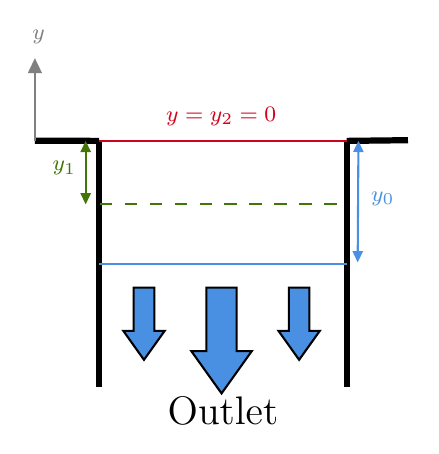
\begin{tikzpicture}[x=0.75pt,y=0.75pt,yscale=-1,xscale=1]
%uncomment if require: \path (0,232); %set diagram left start at 0, and has height of 232

%Straight Lines [id:da2544759348837675] 
\draw [line width=2.25]    (80.96,70) -- (80.96,188.66) ;
%Straight Lines [id:da7574547072545286] 
\draw [line width=2.25]    (200.22,188.66) -- (200.22,70) ;
%Straight Lines [id:da4990218087887346] 
\draw [line width=2.25]    (50,69.91) -- (80.96,70) ;
%Straight Lines [id:da5933583253972261] 
\draw [line width=2.25]    (200.22,70) -- (229.75,69.66) ;
%Straight Lines [id:da9214295287986949] 
\draw [color={rgb, 255:red, 208; green, 2; blue, 27 }  ,draw opacity=1 ]   (80.96,70) -- (200.22,70) ;
%Straight Lines [id:da1922898257916934] 
\draw [color={rgb, 255:red, 65; green, 117; blue, 5 }  ,draw opacity=1 ] [dash pattern={on 4.5pt off 4.5pt}]  (81.33,100.56) -- (200.59,100.56) ;
%Straight Lines [id:da7441027295861509] 
\draw [color={rgb, 255:red, 74; green, 144; blue, 226 }  ,draw opacity=1 ]   (80.96,129.33) -- (200.22,129.33) ;
%Straight Lines [id:da5144800892821806] 
\draw [color={rgb, 255:red, 74; green, 144; blue, 226 }  ,draw opacity=1 ]   (205.86,73) -- (205.53,125.51) ;
\draw [shift={(205.51,128.51)}, rotate = 270.36] [fill={rgb, 255:red, 74; green, 144; blue, 226 }  ,fill opacity=1 ][line width=0.08]  [draw opacity=0] (5.36,-2.57) -- (0,0) -- (5.36,2.57) -- cycle    ;
\draw [shift={(205.88,70)}, rotate = 90.36] [fill={rgb, 255:red, 74; green, 144; blue, 226 }  ,fill opacity=1 ][line width=0.08]  [draw opacity=0] (5.36,-2.57) -- (0,0) -- (5.36,2.57) -- cycle    ;
%Straight Lines [id:da9034738729177096] 
\draw [color={rgb, 255:red, 65; green, 117; blue, 5 }  ,draw opacity=1 ]   (74.46,73) -- (74.46,97.56) ;
\draw [shift={(74.46,100.56)}, rotate = 270] [fill={rgb, 255:red, 65; green, 117; blue, 5 }  ,fill opacity=1 ][line width=0.08]  [draw opacity=0] (5.36,-2.57) -- (0,0) -- (5.36,2.57) -- cycle    ;
\draw [shift={(74.46,70)}, rotate = 90] [fill={rgb, 255:red, 65; green, 117; blue, 5 }  ,fill opacity=1 ][line width=0.08]  [draw opacity=0] (5.36,-2.57) -- (0,0) -- (5.36,2.57) -- cycle    ;
%Straight Lines [id:da8984540196479969] 
\draw [color={rgb, 255:red, 128; green, 128; blue, 128 }  ,draw opacity=1 ]   (50,69.91) -- (50,33.16) ;
\draw [shift={(50,30.16)}, rotate = 90] [fill={rgb, 255:red, 128; green, 128; blue, 128 }  ,fill opacity=1 ][line width=0.08]  [draw opacity=0] (7.14,-3.43) -- (0,0) -- (7.14,3.43) -- cycle    ;
%Right Arrow [id:dp25345861768552247] 
\draw  [fill={rgb, 255:red, 74; green, 144; blue, 226 }  ,fill opacity=1 ] (147.21,140.66) -- (147.21,171.26) -- (154.5,171.26) -- (139.93,191.66) -- (125.36,171.26) -- (132.64,171.26) -- (132.64,140.66) -- cycle ;
%Right Arrow [id:dp07833670135680992] 
\draw  [fill={rgb, 255:red, 74; green, 144; blue, 226 }  ,fill opacity=1 ] (182.28,140.66) -- (182.28,161.54) -- (187.25,161.54) -- (177.3,175.47) -- (167.36,161.54) -- (172.33,161.54) -- (172.33,140.66) -- cycle ;
%Right Arrow [id:dp3532119282431716] 
\draw  [fill={rgb, 255:red, 74; green, 144; blue, 226 }  ,fill opacity=1 ] (107.53,140.66) -- (107.53,161.54) -- (112.5,161.54) -- (102.55,175.47) -- (92.61,161.54) -- (97.58,161.54) -- (97.58,140.66) -- cycle ;

% Text Node
\draw (210.54,97.74) node [anchor=west] [inner sep=0.75pt]  [font=\footnotesize,color={rgb, 255:red, 74; green, 144; blue, 226 }  ,opacity=1 ]  {$y_{0}$};
% Text Node
\draw (139.74,64.37) node [anchor=south] [inner sep=0.75pt]  [font=\footnotesize,color={rgb, 255:red, 208; green, 2; blue, 27 }  ,opacity=1 ]  {$y=y_{2} =0$};
% Text Node
\draw (71.2,83.22) node [anchor=east] [inner sep=0.75pt]  [font=\footnotesize,color={rgb, 255:red, 65; green, 117; blue, 5 }  ,opacity=1 ]  {$y_{1}$};
% Text Node
\draw (140.59,191.66) node [anchor=north] [inner sep=0.75pt]  [font=\Large] [align=left] {Outlet};
% Text Node
\draw (51.74,24.62) node [anchor=south] [inner sep=0.75pt]  [font=\footnotesize,color={rgb, 255:red, 128; green, 128; blue, 128 }  ,opacity=1 ]  {$y$};


\end{tikzpicture}

            \caption{}
            \label{fig:transition-sizes:vein}
        \end{subfigure}
        \caption{(a) Illustrates the semi-minor and semi-major axes defined in Appendix \ref{sec:smooth-transition} for the central cavity transition, including the marked point at the top of the centre of the inlet artery. (b) Illustrates parameters used in defining the smooth transition over the outlet veins.}
        \label{fig:transition-sizes}
    \end{figure}

    The smooth transition regions in the veins are defined using
    \begin{equation*}
        m(\vec{x}) := (\vec{x} - \vec{c}) \cdot \hat{\vec{n}},
    \end{equation*}
    where $\hat{\vec{n}} := \vec{n}/|\vec{n}|$, $\vec{n} = \vec{c} - \vec{p}$, and $\vec{p} \equiv (p_1, p_2)^\intercal$ is the centre of the large circle that traces out the curve on the basal plate. Here, $\vec{c}$ is the point at the centre of where a vein meets the placenta.

    The coefficient $\Psi$ is then given as
    \begin{equation}
        \Psi(\vec{x}) := 
        \begin{cases}
            0, & \text{if } \vec{x} \in \Omega_\text{a} \cup \Omega_\text{CC}, \\
            \beta_{r_0,r_1,r_2}(r(\vec{x})), & \text{if } \vec{x} \in \Omega_{\text{T}^-} \cup \Omega_{\text{T}^+}, \\
            \beta_{y_0,y_1,y_2}(m(\vec{x})), & \text{if } \vec{x} \in \Omega_\text{v}, \\
            1, & \text{if } \vec{x} \in \Omega_\text{IVS}, \\
        \end{cases}
        \label{eq:smooth-transition}
    \end{equation}
    where $y_2 - y_0$ is chosen to give a transition region in the veins with $y_1 \equiv \frac{y_0 + y_2}{2}$, which are shown in Figure \ref{fig:transition-sizes:vein}. A slice of $\Psi(\vec{x})$ on the placentone geometry along $y = 0$ is illustrated in Figure \ref{fig:transition:slice}.
    